\documentclass[a4paper, openright, 12pt]{report}
\usepackage[spanish]{babel}
\usepackage[utf8]{inputenc}
\usepackage{url}
\usepackage{hyperref}
\usepackage{enumerate}
\usepackage{graphicx}
\graphicspath{ {../imgs/} }


\begin{document}


\begin{titlepage}

	\begin{center}
		\vspace*{-1in}
		\begin{figure}[htb]
			\begin{center}
			
\includegraphics[width=3.5cm, height=4cm]{/unam.png}
			\end{center}
		\end{figure}
		\vspace*{0.35in}

		\begin{large}
			\rule{130mm}{0.1mm}\\
			UNIVERSIDAD NACIONAL AUTÓNOMA DE MÉXICO
		\end{large}
		\vspace*{0.55in}

		FACULTAD DE INGENIERÍA \\
		\vspace*{0.25in}
		DEPARTAMENTO DE INGENIERÍA MECÁNICA E INDUSTRIAL\\
		\vspace*{0.6in}
		\begin{large}
			TESIS:\\
		\end{large}
		\vspace*{0.2in}

		\begin{Large}
			\textbf{ Desarrollo de un sistema de detección y manipulación de objetos para un robot de Servicio} \\
		\end{Large}
		\vspace*{0.65in}

		\rule{110mm}{0.1mm}

		\vspace*{0.35in}
		\begin{large}
			Edgar de Jesús Vázquez Silva \\
			\vspace*{0.25in}
			Noviembre 2016\\
		\end{large}


	\end{center}

\end{titlepage}





\tableofcontents{}

\newpage{}
	\section*{Agradecimientos}

	A mi familia,\\
	al laboratorio de Biorobótica\\
	al Dr. Jesús Savage Carmona\\
	al Mtro. Marco Negrete Villanueva\\
	por su paciencia y apoyo en todo momento.\\



	Se agradece al CONACYT, a través del proyecto 24541, "Laboratorio de Movilidad e Infraestructura Verde para la Eficiencia Energética en Ciudades", por el apoyo recibido en la realización de este documento.



\newpage{}
\section*{Abstract}
	En particular, el reconocimiento de objetos y la adecuada manipulación de los mismos es una problemática común en el área de la robótica de servicios. Por ello el presente documento aborda la caracterización de un sistema de manipulación de objetos formado por un brazo robótico de 7DOF, el desarrollo de un algoritmo de visión computacional para reconocer la posición y orientación de los objetos, el desarrollo de la cinemática inversa del brazo robótico y finalmente una metodología de planeación de acciones entre la detección de un objeto y su correcta manipulación.




\chapter{Introducción}
	%¿Por qué son importantes los robots de servicio?
	En los ultimos años el área de la robótica y sus multiples aplicaciones se han expandido a pasos agigantados, tal es el caso de la robótica de servicios. 30 años atrás la idea de tener un robot capáz de ayudar a las tareas del hogar sólo era concebida gracias a la ciencia ficción; hoy en día es una total realidad. Un robot es un sistema mecánico controlado automaticamente, reprogramable, mutiproposito con diversos grados de libertad, el cual puede ser fijo o móvil \cite{khalil2004}. Actualmente existe un auge en utilizar a los robots como auxiliares en las actividades dómesticas, un área támbien llamada: "robots de asistencia o robots de servicio". Sin embargo el área de la robótica de servicios y robots de asistencia comprende un gran rango de problemáticas.\\
	%\vspace{0.2in}

	%¿Cual es la problematica?
	\section{Planteamiento del problema}
		Los robots enfrentan problemáticas a la que cualquier humano está sometido día a día: ámbientes dinámicos, características de entornos no estandarizados, incertidumbre ante escenarios desconocidos. Dada la naturaleza de esta disciplina cientifica han surgido diversas líneas de investigación que abarcan estas problemáticas. Por ejemplo el robot debe ser capaz: de reconocer y manipular objetos en diferentes ubicaciones y desde diferentes alturas, de tener locomoción en diferentes tipos de superficies, de interactúar con un humano, de distinguir diferentes personas. Por último, pero no menos importante, el funcionamiento seguro de estos sistemas en ámbientes dinámicos es un requisito fundamental para su futura aceptación y aplicabilidad.\\
		%\vspace{0.2in}

		%Problemática robots de servicio.
		La creación de estos sistemas autónomos requiere la integración de un gran conjunto de capacidades y tecnologías. Los ejemplos incluyen la interacción humano-robot (habla, identificación de personas, seguimiento de personas, entre otros), navegación, planificación de acciones, control de comportamientos, detección y reconocimiento de objetos, manipulación de objetos o seguimiento de objetos. Con respecto a la inteligencia, los sistemas deben contener métodos de planificaciónde acciones y comportamientos adaptables. Los procedimientos apropiados deberían, por ejemplo, permitir al operador del robot enseñar nuevos comportamientos y entornos vía comandos de voz o gestos. Los futuros hogares probablemente contendrán dispositivos electrónicos más inteligentes capaces de comunicarse entre si incluyendo el uso de internet como base común de conocimientos, de modo que los robots desempeñarán un papel más importante.\\
		%\vspace{0.2in}

		%Problemática de la manipulación
		Entre todas estas líneas de investigación es imprescindible contar con un robot que sea capaz de interactuar con los objetos en el mundo real, por ello es necesario contar un sistema que pueda reconocer los objetos y su posición adecuadamente. Sin embargo esta línea de investigación atiende a problemáticas muy concretas, en el mundo real  los robots se enfrentan con condiciones dinámicas en el ambiente, por ejemplo al pedir a un robot que tome un objeto y pueda llevarlo hasta nosotros el primer problema al que nos enfentamos es conocer la posición del objeto (la cual será diferente en cada ocasión), posteriormente si deseamos localizar dos objetos del mismo tipo estos no serán reconocidos de igual manera por el robot debido a las condiciones de luz, a los cambios de forma, y a los cambios de aparencia.\\
		%\vspace{0.2in}


		%¿Cómo se solucionaria el problema?
		Dadas las características antes descritas, es preciso estimar la probabilidad de que un robot pueda manipular correctamente los objetos. Para ello es necesario dividir la tarea en operaciones: la primera de ellas conciste en estimar la posición del objeto, tener un indicador que nos ayude a determinar cuál es la mejor forma de tomar un objeto y conocer la probalidad de que el robot haya reconocido un objeto exitosamente. Otra de las operaciones necesarias es llevar el actuador final del brazo robótico a una posición (x, y, z) deseada. Por último es necesario contar con un planeador de acciones para coordinar cada uno de los eventos dentro de la tarea.\\
		%\vspace{0.2in}


		Podemos observar que las problematicas son variadas, sin embargo podemos reducir el problema principal en tres tareas secundarias: Detectar un objeto, obtener una aproximación de cuál será la mejor manera de tomarlo y caracterizar el sistema en conjunto para obtener un parámetro de confiabilidad.\\
		%\vspace{0.2in}

		%¿Qué encontraremos en el documento?
		En el capítulo 3 de este documento se aborda la manera en que se desarrollaron los algoritmos de visión computacional para realizar la extracción de un plano, identificar la posición de un objeto, implementar un algoritmo de Análisis de Componentes Principales para obtener cual será la mejor orientación para tomar un objeto a partir de su forma. En el capítulo 4 se describe el sistema de manipulación utilizado. Se comienza por conocer las características de los actuadores utilizados, se obtienen las ecuaciones correspondientes a la cinemática de los brazos para llevarlo hasta una posicón (x, y, z, roll, pitch, yaw) deseda. En el capítulo 5 se realiza la integración de las tareas antes mencionadas, la plataforma sobre la cual se desarrolló el sistema y se describe el desarrollo del modelo probabilístico utilizado para mejorar la manipulación de objetos en un robot de servicios.\\

		Por otra parte, la detección, reconocimiento, localización y seguimiento de objetos, son habilidades básicas con que debe contar un robot de servicio. Existe abundante literatura científica que aborda todos estos problemas aplicando técnicas de inteligencia artificial y visión computacional. Algoritmos como la segmentación por color y profundidad, empatado de nubes de puntos y estimación de posición y velocidad mediante filtros, son ejemplos de algoritmos que pueden abstraerse y estudiarse independientemente de la aplicación en particular. En este trabajo se abordarán estos temas con un enfoque de aplicación en la robótica de servicio, sin embargo, se discutirá sobre la forma en que pueden aplicarse a otros problemas como por ejemplo, la detección de objetos en movimiento en calles y avenidas para el desarrollo de sistemas de navegación autónoma.\\

		Los algoritmos de visión computacional e inteligencia artificial empleados en este trabajo son extrapolables a la detección de objetos como vehículos, peatones y bicicletas. Al final del trabajo se discutirá la forma de aplicarlos en sistemas de planeación de tráfico de vehículos y bicicletas.\\



	\section{Hipótesis}
		\begin{itemize}

			\item Un sistema de visión computacional con implementación de un algoritmo de análisis de componentes principales podrá indicarnos cuál es la mejor orientación para tomar un objeto y por tanto mejorará manipulación de objetos.\\
			%\vspace{0.25in}

		\end{itemize}

	\section{Objetivos}
		\subsection*{Objetivo general}
			Implemetar un conjunto de algoritmos de visión computacional que mejore el sistema de detección y manipulación de objetos formado por un sensor kinect y un brazo robótico de 7DOF en un robot de servicios.
		\subsection*{Objetivos específicos}
			\begin{itemize}
				\item Implementar un algoritmo de visión computacional para identificar un plano.

				\item Implementar un algoritmo de visión computacional para determinar la posición de un objeto.

				\item Implementar un algoritmo de analisis de componentes principales para identificar la orientación de los objetos.

				\item Calcular la cinemática inversa de un brazo robótico de 7DOF para llevarlo a una posición deseada (x, y, z, roll, pitch, yaw).

				\item Caracterizar el sistema de manipulación de objetos usando un modelo bayesiano.

			\end{itemize}




\chapter{Marco teórico}
	\section{Robots de servicio}
		%Conceptos


		%Estado del arte
		Dado que este trabajo se centrará en los robots de servicio, en partícular en una metodología de detección y manipulación de objetos, resulta fundamental poner en evidencia el panorama actual de los robots de servicio. La idea general de la robótica de servicio doméstico ha existido desde hace mucho tiempo, pero es un tema de investigación relativamente joven. El objetivo de crear robots de servicios útiles y autónomos que puedan interactuar con seres humanos y objetos en el mundo real en un entorno natural plantea un gran número de problemas sin resolver en muchas disciplinas científicas.\\
		%\vspace{0.2in}

		Recientemente, el progreso en estos campos de investigación, así como el progreso y la normalización en el desarrollo de hardware y software, ha llevado a un aumento en la disponibilidad de recursos, métodos y componentes para el desarrollo  de Robots de servicio doméstico . Por ello estamos cada vez más cerca de convivir con robots de servicios de manera exitosa en diversos lugares, por ejemplo hospitales \cite{hospitalRobots}, oficinas, construcciones, o tiendas departamentales \cite{robotsInStores}.\\
		%\vspace{0.2in}


		Estos desarrollos han sido posibles gracias a herramientas de código abierto como lo es Ubuntu, ya que ha servido como base para el desarrollo de software especializado para robots, por ejemplo ROS \cite{rosEpage}. Este conjunto de librerías especializadas para robots pueden llegar a ser muy patículares y estar enfocados a una sola área de invetigación de las antes mencionadas, por ejemplo: Carmen \cite{carnegieMellon}, un conjuto de liberías y algoritmos de control para navegación de robots, desarrollados por la universidad Carnegie Mellon\cite{cMellonEpage}.\\
		%\vspace{0.2in}

		En la parte de simulación se cuenta con ejemplos como el USARSim \cite{balakirsky2006}, rviz \cite{rVizEpage} o Gazebo \cite{gazeboEpage}. Por lo que respecta a los algoritmos de visión computacional existen bibliotecas de código abierto por ejemplo OpenCV \cite{openCV} el cual tiene un gran campo de aplicaciones\cite{bradski2000}. Por lo que corresponde a los kits standar de hardware, podemos mencionar la construcción de robots de plataforma standar por ejemplo VolksBot \cite{wisspeintner2007} y las plataformas bases por ejemplo ActivRobots \cite{ActivRobots}, Pepper \cite{pepperEpage}, Asimo \cite{asimoEpage} ha hecho posible desarrollar software de manera más rápida y eficiente.\\
		%\vspace{0.2in}

		\begin{figure}[htb]
			\begin{center}
			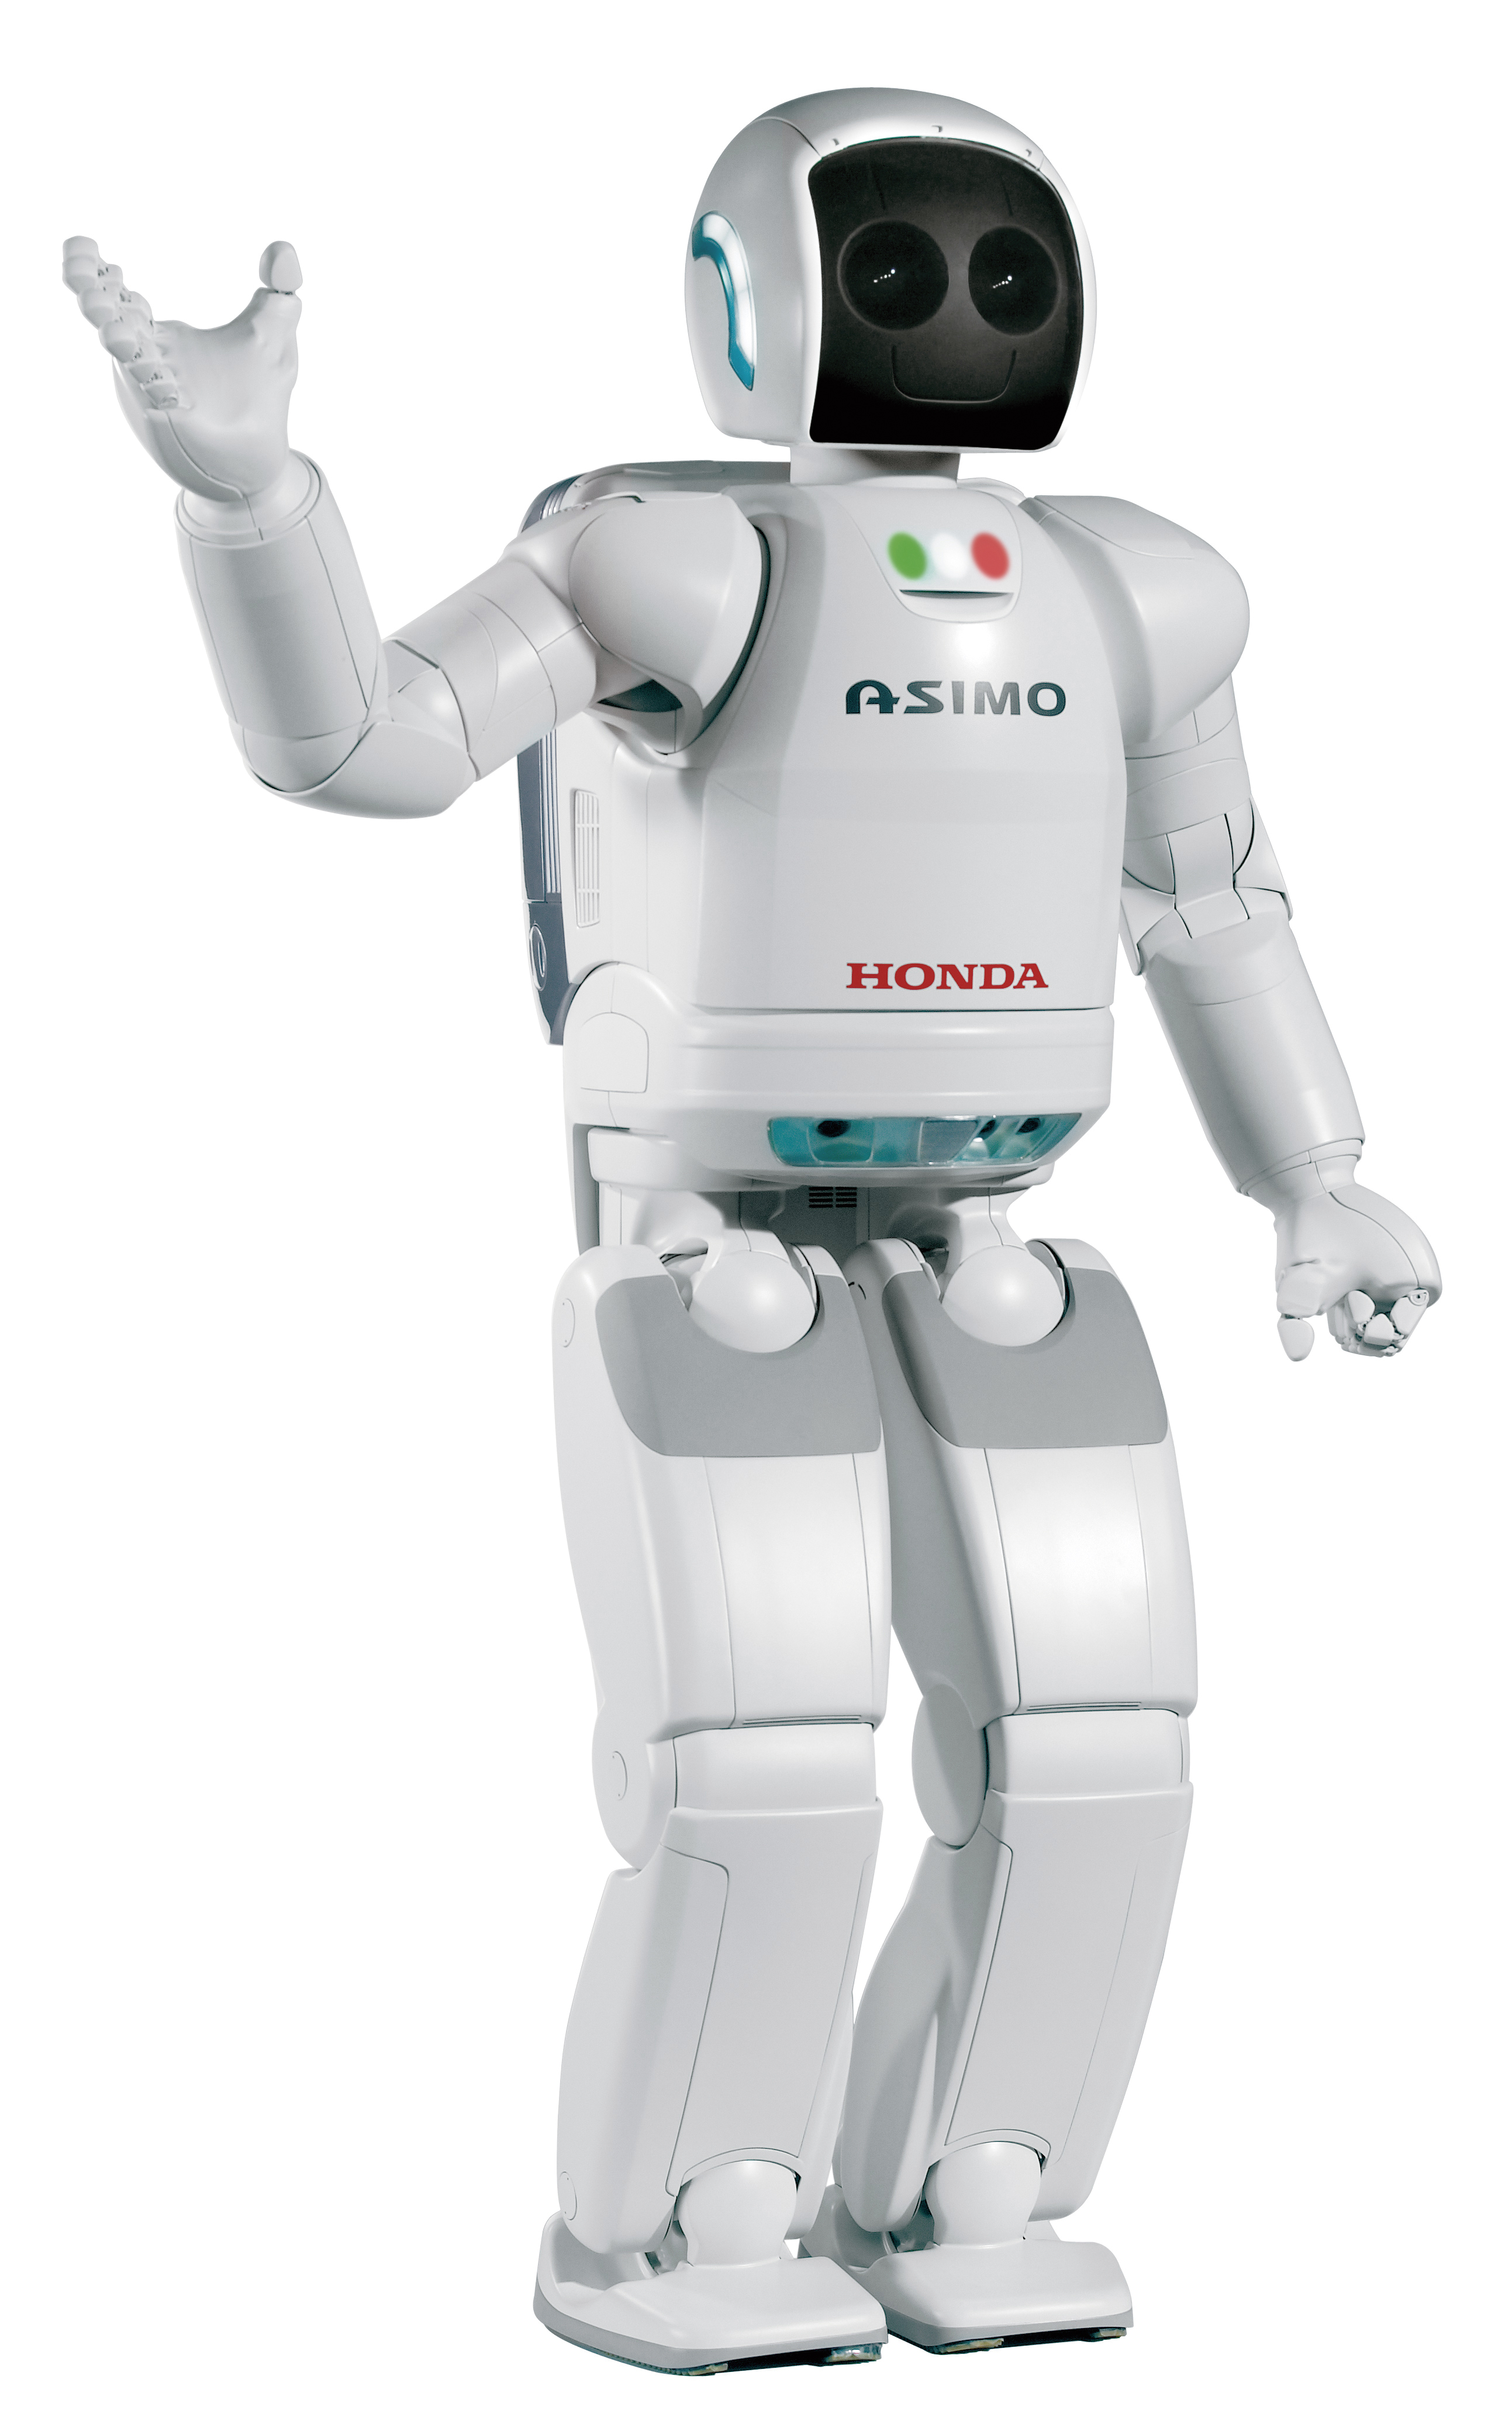
\includegraphics[width=3.5cm, height=5cm]{/asimo.jpg}
			\end{center}
		\end{figure}



%%% Fundamentos de Manipuladores
%%  ---------------------------------

	\section{Fundamentos básicos de Robots Manipuladores}
		La manipulación adecuada de objetos es una característica imprescindible en los robots de servicio dadas las condiciones de su entorno y las tareas cotidianas que le podemos asignar a dicho robot. Una posible solución a la problemática de la manipulación de objetos es la incorporación de manipuladores seriales a una base móvil; sin embargo se debe tener encuenta que los objetos a ser manipulados se encuentran en condiciones aleatorias de posición y orientación, estas características implican que el manipulador serial debería ser capaz de alcanzar una posición (x, y, z) con cualquier orientación (roll, pitch, yaw).\\

		Los robots manipuladores clásicos presentan una configuración antropomórfica serial, que hace semejanza con un brazo humano. La arquitectura típica de un manipulador consiste en una serie de barras rígidas unidas entre sí mediante el uso de acticulaciones rotacionales o prismáticas. De manera general cada articulación logra su movimiento gracias a un actuador y a la adición de algunos elelmentos complementarios como sensores de posición y de velocidad\cite{baturone2005}.\\

		*Los robots manipuladores clásicos están caracterizados, desde el punto de vista mecánico, por una serie de propiedades talez como los grados de libertad, el espacio de trabajo, la rígidez estructural, repetitibilidad y peso propio. Además en los robots manipuladores suelen tomarse en cuenta otras características adicionales: la carga útil máxima y la velocidad de trabajo.\\

		\begin{figure}[htb]
			\begin{center}
			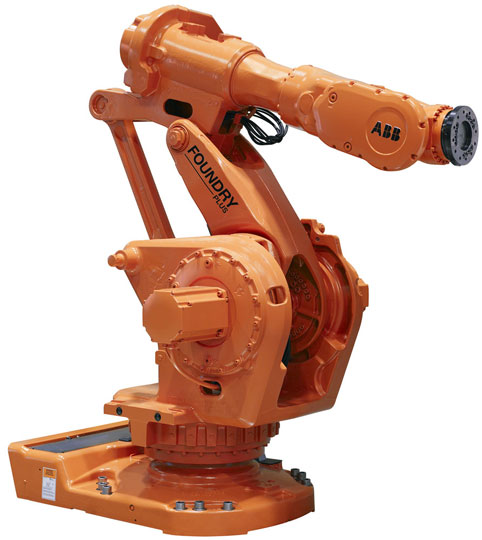
\includegraphics[width=3.5cm, height=4cm]{/serial_abb.jpg}
			\end{center}
		\end{figure}

		\subsection{Configuraciones típicas y parámetros característicos}
			****Según la geometría de su estructura mecánica, un manipulador puede ser:

			\begin{itemize}
				\item{Cartesiano, cuyo posicionamiento en el espacio se lleva a cabo mediante articulaciones lineales.}

				\item{Cilíndrico, con una articulación rotacional sobre una base y articulaciones lineales para el movimiento en altura y en radio.}

				\item{Polar, que cuenta con dos articulaciones rotacionales y una lineal.}

				\item{Esférico (o de brazo articulado), con tres articulaciones rotacionales.}

				\item{Mixto, que posee varios tipos de articulaciones, combinaciones de las anteriores. Es destacable la configuración SCARA (Selective Compliance Assembly Robot Arm).}

				\item{Paralelo, posee brazos con articulaciones prismáticas o rotacionales concurrentes.}
			\end{itemize}

Los principales parámetros que caracterizan a los robots industriales son:

	\begin{itemize}
		\item{Número de grados de libertad. Es el número total de grados de libertad de un robot, dado por la suma de g.d.l. de las articulaciones que lo componen. Aunque la mayoría de las aplicaciones industriales requieren 6 g.d.l., como las de soldadura, mecanizado y almacenamiento, otras más complejas requieren un número mayor, tal es el caso de las labores de montaje.}

		\item{Espacio de accesibilidad o espacio (volumen) de trabajo. Es el conjunto de puntos del espacio accesibles al punto terminal, que depende de la configuración geométrica del manipulador. Un punto del espacio se dice totalmente accesible si el PT puede situarse en él en todas las orientaciones que permita la constitución del manipulador y se dice parcialmente accesible si es accesible por el PT pero no en todas las orientaciones posibles. En la figura inferior se aprecia el volumen de trabajo de robots de distintas configuraciones.}

		\item{Capacidad de posicionamiento del punto terminal. Se concreta en tres magnitudes fundamentales: resolución espacial, precisión y repetibilidad, que miden el grado de exactitud en la realización de los movimientos de un manipulador al realizar una tarea programada.}

		\item{Capacidad de carga. Es el peso que puede transportar el elemento terminal del manipulador. Es una de las características que más se tienen en cuenta en la selección de un robot dependiendo de la tarea a la que se destine.}

		\item{Velocidad. Es la máxima velocidad que alcanzan el PT y las articulaciones.}
	\end{itemize}

		\begin{figure}[htb]
			\begin{center}
			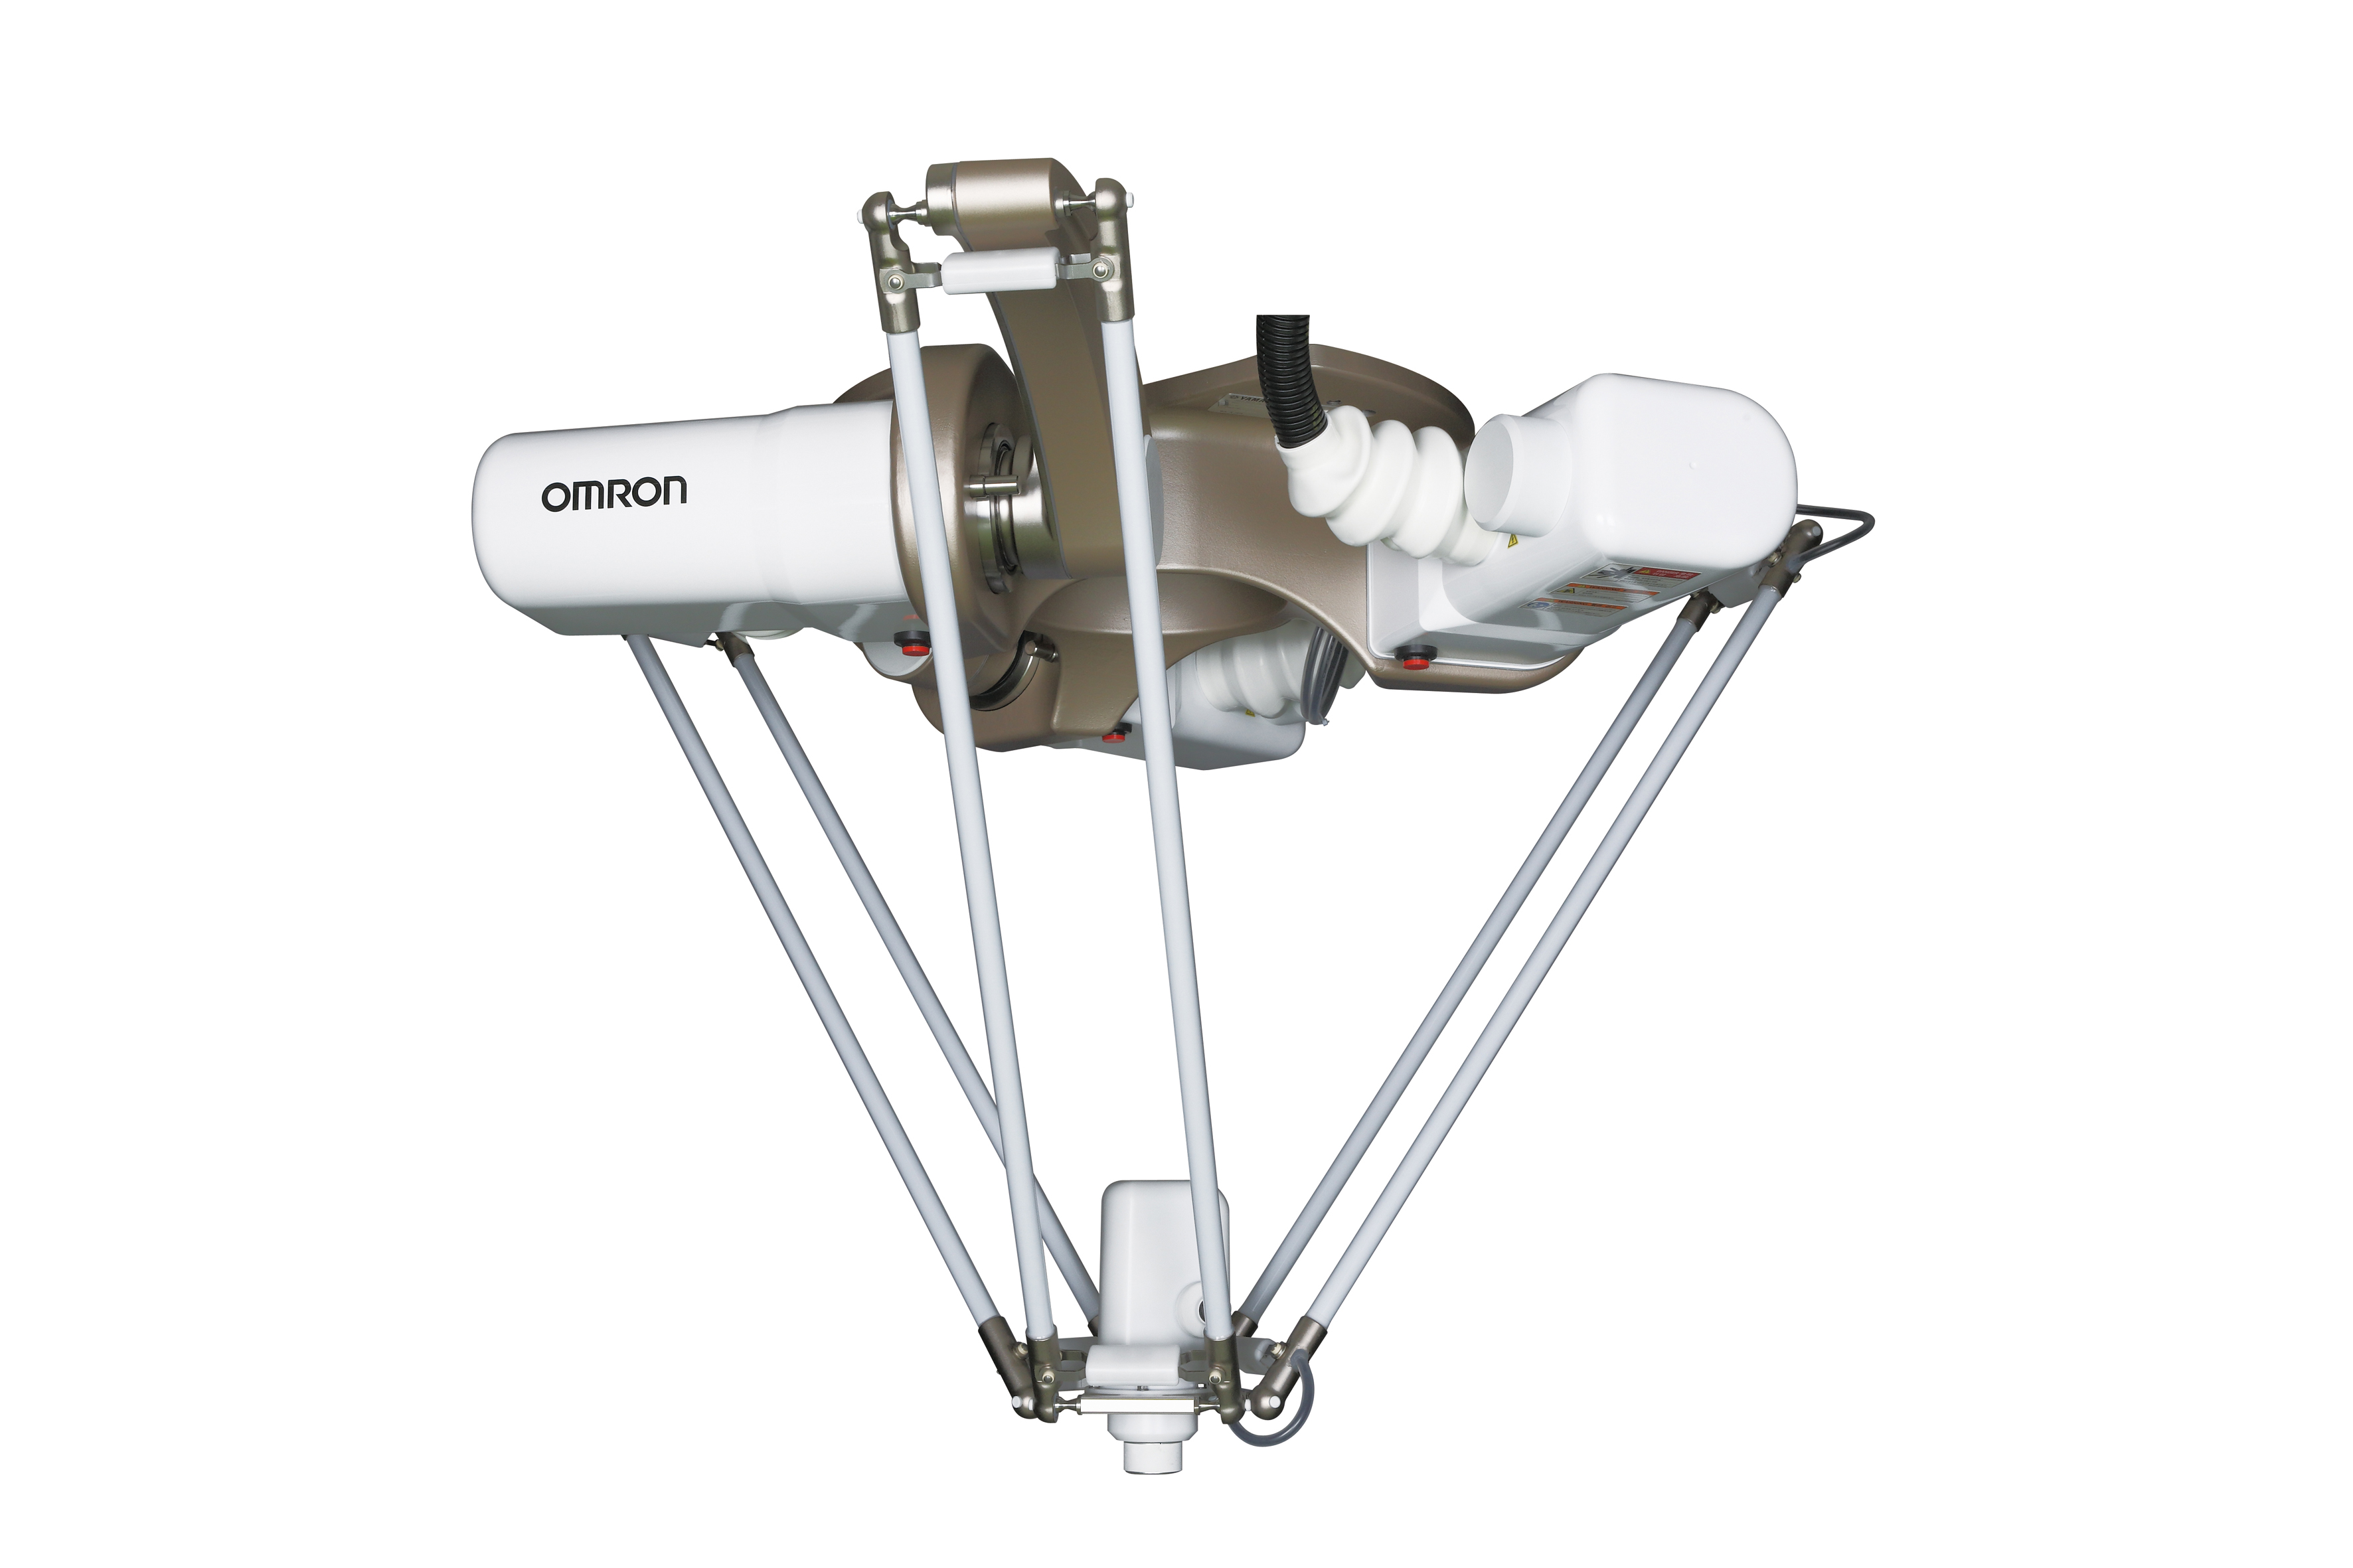
\includegraphics[width=6.5cm, height=4.5cm]{/robotParalelo.jpg}
			\end{center}
		\end{figure}


		\subsection{Descripciones espaciales y transformaciones}
			*La cinemática es la ciencia del movimiento que trata el tema sin considerar las fuerzas que lo ocasionan. Dentro de esta ciencia se estudian la posición, la velocidad y la aceleración. En conseciencia, el estudio de la cinemática de manipuladores se refiere a todas las propiedades geométricas y las basadas en los cambios de estas a lo largo del tiempo. Dadas las características de este trabajo solo se abordarán la cinemática directa e inversa, sin llegar a analizar la dinámica del manipulador.\\

			*El problema de la cinemática directa se plantea en términos de encontrar una matriz de trasformación que relaciona el sistema de coordenadas ligado al cuerpo en movimiento respecto a un sistema de coordenadas que permanece estático y se toma como referencia. Para lograr esta representación se usan la matriz de transformación homogénena con una dimension 4x4, la cual incluye las operaciones de rotación y translación.\\

			*La matriz de transformación homogénea es una matriz de 4x4 que trasnforma un vector expresado en coordenadas homogéneas desde un sistema de coordenadas hasta otro sistema de coordenadas. La matriz de transformación homogénea tiene la siguiente estructura:\\

			***Matriz Transformación Homogénea

			donde los vectores n, s, a, son vectores ortogonales unitarios y p es un vector que describe la posición x, y, z del origen del sistema actual respecto del sistema de referencia.

			*** Gráfico sistemas de referencia.







%%  Imagenes RGD y Points Clouds
%%  ----------------------------------------------
	\section{Imágenes RGB-D}
		En la robótica de servicios resulta imprescindible contar con robots que sean capacez de percibir su entorno, los elementos que los rodean y determinar características de los mismos. Los humanos, dadas estas necesidades, hemos desarrollado el sentido de la vista que nos permite determinar características del entorno y de los objetos que lo componen tales como el color, la forma, las dimensiones o su ubicación en el espacio.\\

		En este sentido la visión artificial es la disciplina encargada de estudiar los procesos de reconocer y localizar objetos en el entorno. Entender estos procesos nos ayudará a construir máquinas con capacidades similares.\\


		\subsection{Características de las imágenes RGB-D}



	\section{Algoritmo RANSAC}
	\section{Algoritmo PCA}
	\section{Características del objeto}


	\section{Planeación de tareas}



\chapter{Detección de objetos}
	\section{Kinect}
	\section{OpenCV}
	\section{Algoritmo RANSAC}
	\section{Analísis de componentes principales}


\chapter{Manipulador}
	\section{Descripción de los elementos del sistema de manipulación}
	\section{Documentación servos dynamixel}
	\section{Cinemática inversa}


\chapter{Integración}
	\section{Máquinas de estados}
	\section{ROS}
	\section{Constitución del robot de servicio Justina}


\chapter{Resultados}


\chapter{Conclusiones}


\newpage{}


\bibliographystyle{ieeetr}
\bibliography{biblio.bib}



\end{document}

